\documentclass{beamer}

\usepackage[utf8]{inputenc}
\usepackage[slovene]{babel}
\usepackage{default}
\usepackage{graphicx}
\usepackage{amsmath}
\usepackage{overpic}
\usepackage{geometry}
\usepackage{subfigure}

\renewcommand{\thesubfigure}{}

\usepackage{tikz}
\usetikzlibrary{calc}

\tikzset{egrid/.style={draw,help lines}}
\tikzset{mgrid/.style={draw,help lines,dashed}}
\tikzset{epoint/.style={draw,circle,red,inner sep=2pt,fill}}
\tikzset{mpoint/.style={draw,circle,blue,inner sep=2pt,fill}}

\usetheme{Madrid}

\newcommand{\odvod}[2]{\frac{\partial #1}{\partial #2}}
\renewcommand{\vec}{\mathbf}
\newcommand{\eps}{\varepsilon}
\newcommand{\E}{\vec E}
\newcommand{\B}{\vec B}
\newcommand{\angl}[1]{(\textit{angl. #1})}

\newcommand{\stalno}[2]{
  \begin{overpic}[width=.23\textwidth,trim=-1cm -1cm -1cm -1cm]{g_defect_#2}\end{overpic} 
  \begin{overpic}[width=.23\textwidth]{./Slike/lic_#1_1}\put(2,88){\color{white} \large \bf 1 $\boldsymbol\mu$m}\end{overpic} 
  \begin{overpic}[width=.23\textwidth]{./Slike/lic_#1_37}\put(2,88){\color{white} \large \bf 10 $\boldsymbol\mu$m}\end{overpic} 	
  \begin{overpic}[width=.23\textwidth]{./Slike/lic_#1_50}\put(2,88){\color{white} \large \bf 15 $\boldsymbol\mu$m}\end{overpic}
}

\begin{document}
\title[Zagovor magisterija]{Modeliranje \v sirjenja svetlobe vzdol\v z ograjenih teko\v cekristalnih defektnih linij}
\author[Miha \v Can\v cula]{\begin{tabular}{rl}Avtor & Miha \v Can\v cula \\ Mentor & prof. dr. Slobodan \v Zumer \\ Somentor & doc. dr. Miha Ravnik\end{tabular}}

\date{3. september 2013}

\section{Uvod}

\begin{frame}
 \titlepage
\end{frame}

\begin{frame}{Teko"ci kristali}
 \begin{columns}[c]
  \begin{column}{.5\textwidth}
  
   \begin{itemize}
    \item Lastnosti teko"cin in kristalov
    \item Orientacijski red
      \begin{itemize}
	\item Direktor $\vec n$
	\item Stopnja reda $S$
	\item Simetrija $\vec n \leftrightarrow -\vec n$
      \end{itemize}
    \item Dvolomnost
    \item Delni pozicijski red
    \item Nadzor z zunanjimi polji
    \item Elasti"cne deformacije direktorja
   \end{itemize}
  \end{column}

  \begin{column}{.5\textwidth}
    \includegraphics[width=\textwidth]{./Slike/faze_brez_crk} \\

  \resizebox{\textwidth}{!}{\begin{picture}(400, 120)
    \put(0,30){\includegraphics[height=80pt]{./Slike/fig_frank_components_splay_s}}
    \put(150,20){\includegraphics[height=100pt]{./Slike/fig_frank_components_twist_s}}
    \put(270,30){\includegraphics[height=80pt]{./Slike/fig_frank_components_bend_s}}
    \put(50, 10){\LARGE $\nabla \cdot \vec n$}
    \put(170, 10){\LARGE $\vec n \cdot \nabla \times \vec n$}
    \put(300, 10){\LARGE $\vec n \times \nabla \times \vec n$}
  \end{picture}}
  \end{column}
    
  \end{columns}
  
  \begin{center}
   \includegraphics[height=60pt]{./Slike/cp-1} \,
   \includegraphics[height=60pt]{./Slike/tvorjenje} \,
   \includegraphics[height=60pt]{./Slike/ilcs_03} \,
   \includegraphics[height=60pt]{./Slike/Flat-panel-display-lcd-monitor}
  \end{center}

  
\end{frame}

\begin{frame}{Elektromagnetno valovanje}
\begin{columns}

\column{.6\textwidth}
 
\begin{block}{Maxwellove ena"cbe}
\begin{equation*}
\begin{aligned}
 \nabla \cdot \vec D = \rho_f & \qquad \nabla \cdot \vec B = 0 \\
 \nabla \times \vec E = -\odvod{\vec B}{t} & \qquad \nabla \times \vec H = \vec J_f + \odvod{\vec D}{t}
\end{aligned} 
\end{equation*}
\end{block}

\begin{block}{Konstitutivni zvezi}
\begin{equation*}
\begin{aligned}
\vec D = \boldsymbol\varepsilon \varepsilon_0 \vec E \qquad \vec B = \boldsymbol \mu \mu_0 \vec H
\end{aligned} 
\end{equation*}
\end{block}

\begin{itemize}
 \item $\boldsymbol\eps$ in $\boldsymbol\mu$ sta anizotropna tenzorja
 \item Ohmov zakon $\vec J = \sigma \vec E$
 \item V vzorcu ni prostih nabojev ($\rho_f = 0$)
 \item Izredna os vzporedna z direktorjem
\end{itemize}

\column{.35\textwidth}
\begin{block}{Dvolomnost}
\begin{itemize}
 \item Lomni koli"cnik odvisen od polarizacije svetlobe
 \item Ena izredna os z $n_e$ pravokotne smeri $n_o$
\end{itemize}
\end{block}

\begin{center}
\includegraphics[width=.8\textwidth]{./Slike/Rays_passing_through_birefringent_material}
\end{center}

\end{columns}
\end{frame}

\begin{frame}{Defekti}
 \includegraphics[width=.25\textwidth]{g_defect_2}
 \includegraphics[width=.25\textwidth]{g_defect_-2}
 \includegraphics[width=.25\textwidth]{g_defect_1}
 \includegraphics[width=.25\textwidth]{g_defect_-1}

 \begin{itemize}
  \item Obmo"cje zmanj"sanega reda
  \item Ovojno "stevilo -- celo za vektorska polja, polcelo za direktor
 \end{itemize}
 
 \begin{center}
 \includegraphics[height=100pt]{./Slike/1_v6} \qquad
 \begin{overpic}[height=100pt]{./Slike/defekt-kapljica.png}
  \put(-80,4) {\rotatebox{90}{\tiny Porenta et al., Soft Matter (2012)}}
  \put(10,15) {\tiny Brasselet et al., PRL (2009)}
  \end{overpic}

 \end{center}
 
\end{frame}

\section{Metoda}

\begin{frame}{Numeri"cna metoda}
 \begin{block}{Metoda kon"cnih diferenc v "casovni domeni -- FDTD}
  \begin{itemize}
   \item "Casovni razvoj vseh 6 komponent $\vec E$ in $\vec B$
   \item Dinami"cni Maxwellovi ena"cbi na diskretni mre"zi
   \begin{equation*}
     \odvod{\vec{B}}{t} = -\nabla \times \vec{E} \qquad \odvod{\vec{E}}{t} = \eps^{-1} (\nabla \times \vec{B} - \sigma \vec E)
   \end{equation*}
  \end{itemize}
 \end{block}
 
 \begin{columns}
  \column{.65\textwidth}
   \begin{block}{Diskretizacija na mre"zi}
    \begin{itemize}
	\item Komponente polj znane na razli"cnih krajih ob razli"cnih "casih
	\item Izvor in absorpcija valovanja na robu
      \end{itemize}
    \end{block}
    
    \column{.3\textwidth}
    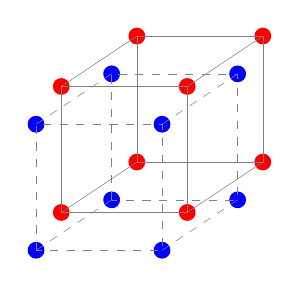
\begin{tikzpicture}[scale=0.8]
    
    \foreach \x in {0,1}{
      \foreach \y in {0,1}{
        \node[mpoint] at (2*\x,2*\y) {}; 
        \node[mpoint] at (2*\x+1.2,2*\y+0.8) {}; 
        \node[epoint] at (2*\x+1.6,2*\y+1.4) {};
        \node[epoint] at (2*\x+1.6-1.2,2*\y+1.4-0.8) {};
        \draw[mgrid] (2*\x,2*\y) -- (2*\x+1.2,2*\y+0.8);
        \draw[egrid] (2*\x+1.6,2*\y+1.4) -- (2*\x+1.6-1.2,2*\y+1.4-0.8);
      }
    }
    
    \draw[mgrid] (0,0) rectangle (2,2);
    \draw[mgrid] (1.2,0.8) rectangle (3.2,2.8);
    \draw[egrid] (1.6,1.4) rectangle (3.6,3.4);
    \draw[egrid] (1.6-1.2,1.4-0.8) rectangle (3.6-1.2,3.4-0.8);

            \end{tikzpicture}

 \end{columns}
\end{frame}

\begin{frame}{Primeri uporabe metode}
\begin{columns}[c]

\begin{column}[T]{.5\textwidth}
\begin{itemize}
 \item "Sirjenje po praznem prostoru
 \includegraphics[width=.9\textwidth]{./Slike/empty}
 
 \item Lom pri Brewsterjevem kotu
 
\includegraphics[width=.9\textwidth]{./Slike/refraction}

 \item Fotonski kristal

\end{itemize}

\end{column}

\begin{column}[T]{.5\textwidth}
\begin{itemize}
  \item Uniformen dvolomni kristal \\
  \hspace{-.5cm}\resizebox{.9\textwidth}{!}{\input{g_test_uniform_nocite}}
  
 \item Dvolomno vlakno
  \includegraphics[width=.41\textwidth]{./Slike/licp_0_68} \hspace{2pt}
  \includegraphics[width=.41\textwidth]{./Slike/licp_0_78}
\end{itemize}

\end{column}

\end{columns}

\end{frame}

\section{Rezultati}

\begin{frame}{Vlakno z radialnim direktorskim profilom}
 \begin{center}

\includegraphics[height=.2\textwidth]{./Slike/radial-cross} \quad

\includegraphics[height=.2\textwidth]{./Slike/director-profile-radial}
\end{center}

 \begin{center}
 \includegraphics[height=.35\textwidth]{./Slike/tvorjenje}\,
 \begin{overpic}[height=.35\textwidth]{./Slike/tvorjenje2}
     \put(103, 10) {\rotatebox{90}{\tiny Peddireddy et al., Langmuir (2012)}}
\end{overpic}
\end{center}

\end{frame}

\begin{frame}{Sunek v vlaknu z radialnim direktorskim profilom}

 \begin{center}
 \includegraphics[width=.4\textwidth]{./Slike/licp_p1_74}\quad
  \includegraphics[width=.4\textwidth]{./Slike/licp_p1_82}
\end{center}

\begin{itemize}
 \item Sunek razpade na dva stacionarna na"cina -- redni in izredni
 \item Temna obmo"cja zaradi vpadne polarizacije
 \item ``Neprava'' defekta z ovojnim "stevilom $+1$
\end{itemize}

\end{frame}

\begin{frame}{Sunek v vlaknih z razli"cnimi defekti}

 \begin{center}
  \includegraphics[height=.35\textheight]{./Slike/licp_m1_74} \quad
  \includegraphics[height=.35\textheight]{./Slike/licp_p12_68} \quad
  \includegraphics[height=.35\textheight]{./Slike/licp_m12_68} \\
  \includegraphics[height=.35\textheight]{./Slike/licp_m1_82} \quad
  \includegraphics[height=.35\textheight]{./Slike/licp_p12_78} \quad
  \includegraphics[height=.35\textheight]{./Slike/licp_m12_78}
\end{center}

\end{frame}

\begin{frame}{Stalna laserska svetloba}
  \stalno{p1}{2} \\[-3.3mm]
  \hrulefill \\[1mm]
  \stalno{p12}{1}
\end{frame}


\begin{frame}{Stalna laserska svetloba}
 \begin{itemize}
  \item Kombinacija dveh stacionarnih na"cinov, razli"cni hitrosti
  \item Stacionarno stanje, polje na vsakem mestu niha
  \item Pretvorba v radialno polarizirano svetlobo
  \item Brez temnih ravnin -- obrat polarizacije za 90$^{\circ}$
 \end{itemize}
 
 \begin{figure}[h]
 \centering
    \subfigure[sunek]{\includegraphics[width=.3\textwidth]{./Slike/licp_p1_82}} \hspace{.3cm}
    \raisebox{.13\textwidth}{\Huge $\boldsymbol\neq$} \hspace{.2cm}
    \subfigure[stalna svetloba]{\includegraphics[width=.3\textwidth]{./Slike/lic_p12_50}}

    
 \end{figure}
 
\end{frame}

\section{Zaklju"cek}

\begin{frame}{Nadaljnje raziskave}
\begin{columns}

\column{.65\textwidth}
 
 \begin{block}{Numeri"cna metoda}
  \begin{itemize}
   \item Sklopitev med svetlobo in teko"cim kristalom
   \item Teko"cekristalne kapljice in vlakna kot laserji
   \item Metamateriali -- zapletene strukture
   \item Natan"cne transmisijske slike
   \item Povezava med teorijo in eksperimenti
  \end{itemize}
 \end{block}
 
 \begin{block}{Teko"cekristalna vlakna}
  \begin{itemize}
    \item Pretvorba polarizacije svetlobe
    \item Opti"cne komunikacije
    \item Laserska svetloba v vse smeri
  \end{itemize}
 \end{block}
 
 
\column{.25\textwidth}

\includegraphics[width=\textwidth, clip, trim=0 22pt 0pt 50pt]{./Slike/CoverIssue48.jpeg} \\[5mm]
\begin{overpic}[angle=90,width=\textwidth]{./Slike/laser-droplet}
\put(70,8) {\rotatebox{90}{\tiny Humar, Mu"sevi"c, Optics Express (2010)}}
\put(70,109) {\rotatebox{90}{\tiny Se"c et al., Soft Matter (2012)}}
\end{overpic}
 
\end{columns}
\end{frame}


\end{document}
